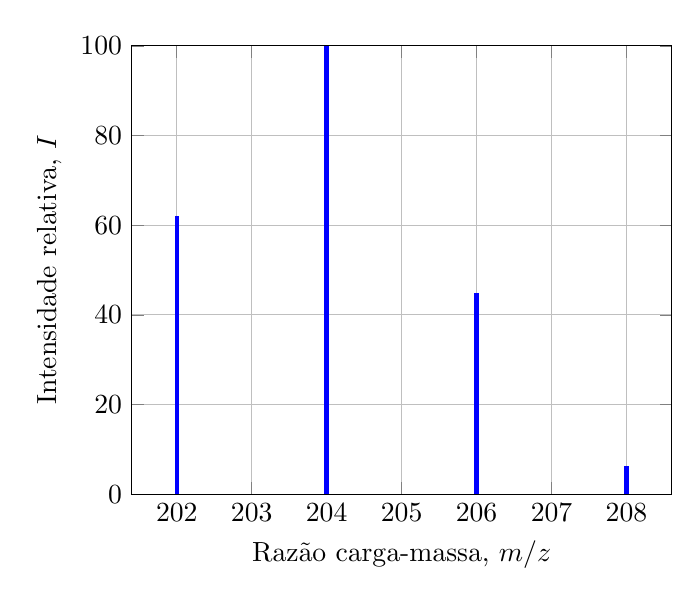
\begin{tikzpicture}
    \begin{axis}
        [
            grid = major,
            ylabel = {Intensidade relativa, $I$},
            xlabel = {Razão carga-massa, $m/z$},
            ymin = 0,
            ymax = 100,
        ]
    \addplot[blue, ultra thick, mark=none] coordinates
        {
            (202, 00)
            (202, 62.008151)
        };
    \addplot[blue, ultra thick, mark=none] coordinates
        {
            (204, 00)
            (204, 100)
        };
    \addplot[blue, ultra thick, mark=none] coordinates
        {
            (206, 00)
            (206, 44.947677)
        };
    \addplot[blue, ultra thick, mark=none] coordinates
        {
            (208, 00)
            (208, 6.175140)
        };
    \end{axis}
\end{tikzpicture}